\documentclass{article}
\usepackage{amsfonts}
\usepackage{graphicx}
\usepackage{enumitem}
\usepackage{amsmath}
\usepackage{float}
\usepackage{tfrupee}
\usepackage{gensymb}
\begin{document}
\begin{enumerate}
\item if $x=3$ is one root of the quadratic equation $x^2-2kx-6$ then find the value of k
\item what is the HCF of smallest prime number and the smallest composite number
\item find the distance of a point $p(x,y)$ from the origin
\item In an $AP$,if the common difference $(d)=-4$,and the seventh term $(a_{7})$ is $4$,then find the first term
\item what is the value of $(\cos^2{67^\circ}$-$\sin^2{23^\circ})$
\item Given $\Delta ABC ~ \Delta PQR$,if $\frac{AB}{PQ}$=$\frac{1}{3}$ then find $\frac {ar \Delta ABC}{ar \Delta PQR}$
\item Given that $\sqrt{2}$ is irrotational,prove that $(5+\sqrt[3]{2})$ is an irrotational number
\item In fig $1$,$ABCD$ is a rectangule.Find the values of $x$ and $y$\\
	\begin{figure}[H]
		\centering
		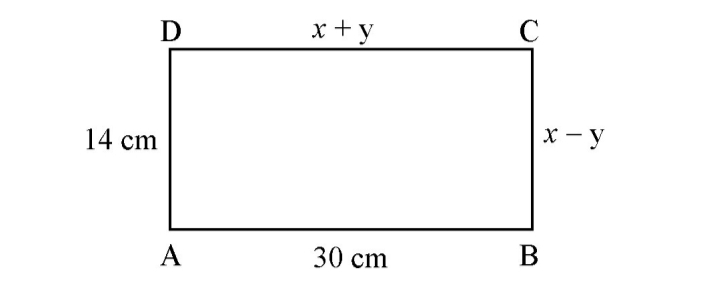
\includegraphics [width=\columnwidth] {./IMG1.jpg}
		\label{fig:fig1}
		\caption{rectangular ABCD}
	\end{figure}
\item Find the sum of first $8$multiples of $3$
\item Find the ratio in which $p(4,m)$ divides the line segment joining the points $A(2,3)$ and $b(6,-3)$.Hence find m
\item Two different dice are tossed together.find the probability;
	\begin{enumerate}[label=\roman*)]
		\item of getting a doublet
		\item of getting a sum $10$,of the numbers on the two dice
	\end{enumerate}
\item An integer is chosen at random between $1$ and $100$.find the probability that it is:
	\begin{enumerate}[label=\roman*)]
		\item divisible by $8$
		\item not divisible by $8$
	\end{enumerate}
\item Find HCF and LCM of $404$ and $96$ and verify that $HCF \times LCM =$ product of two given numbers
		\item Find the zeros of the polynomial$(2x^4-9x^3+3x-1)$.if two of its zeros are $(2+\sqrt+3)$ and $(2-\sqrt+3)$
		\item If $A(-2,1)$,$B(a,0)$,$C(4,b)$ and $D(1,2)$ are the vertices of a parallelogram ABCD,find the values of a and b.Hence find the length of its sides\\
										(or)\\
			If $A(-5,7)$,$B(-4,-5)$,$C(-1,-6)$ and $D(4,5)$ are the vertices of a quadrilateral,find the are of the quadrilateral ABCD
		\item A plane left $30 minutes$ late than its scheduled time and in order to reach the destination $1500km$ away in time,it had to increase its speed by $100km/h$ from the usual speed.find its usual speed.
		\item prove that the area of n equilateral triangle described on one side of the square is equal to half the area of the equilateral triangle described on one of its diadonal\\
			(or)\\
			If the area of two similar triangles are equal.prove that they are congruent
		\item prove that the lengths of tangents drawn from an external point to a circle are equal
		\item if $4\tan\theta=3$,evaluate$(\frac {4\sin\theta-\cos\theta+1} {4\sin\theta+\cos\theta-1})$\\
			(or)\\
			If $( \tan 2A)$ = $\cot(A - 18\degree)$ \ where \( 2A \) is an acute angle, find the value of \( A \). 
		\item Find the area of the shaded region in fig 2,where areas drawn with centers A,B,C and D intersect in pair at mid-points.P,Q,R and S of the sides AB,BC,CD and DA respectively of a square ABCD of side $12cm$.$[use \pi=3.14]$ \\

			\begin{figure}[H]
			\centering
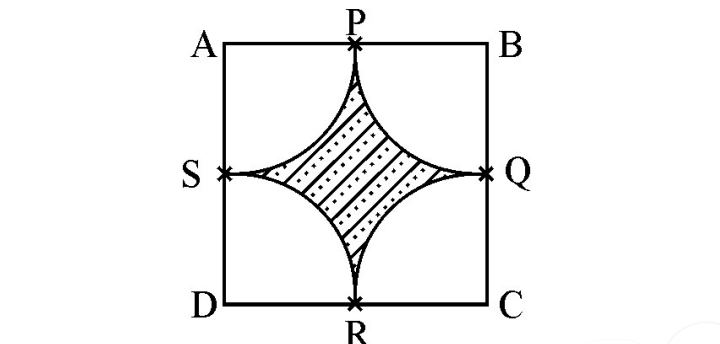
\includegraphics [width=\columnwidth] {./IMG3.jpg} 
		\label{fig:fig2}
\caption{square ABCD} 
\end{figure}
	

		\item A wooden article was made by scooping out a hemisphere from each end of a slid cylinder,as shown in fg 3.if the height of the cylinder is $10cm$ and its base is of eadius $3.5cm$.find the total surface area of the article.\\
			\begin{figure}[H]                                                            \centering                                                             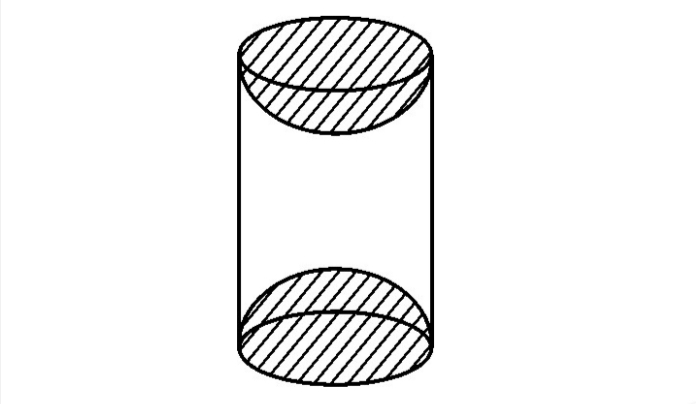
\includegraphics [width=\columnwidth] {./IMG2.jpg}                     \label{fig:fig1}                                                       \caption{cylinder}
			\end{figure}

	\item The table below shows the salaries of $280$ persons\\     \begin{tabular}{|c|c|}                                                                        \hline                                                                 (Salary in thousand\rupee) & No of persons\\ \hline                                                                                           $5-10$ & $49$\\ \hline                                                 $10-15$ & $133$\\ \hline                                               $15-20$ & $63$\\ \hline                                                $20-25$ & $15$\\ \hline                                                $25-30$ & $6$\\ \hline                                                 $30-35$ & $7$\\ \hline                                                 $35-40$ & $4$\\ \hline                                                 $40-45$ & $2$\\ \hline                                                 $45-50$ & $1$\\ \hline                                         \end{tabular}\\                                                        Calculate the median salary of the data.
					
	\item A motor boat whose speed is $18 km/hr$ in still water takes $1hr$ more to go $24km$ upstream than to return down stream to the same spot.Find the speed of the stream.\\
		(OR)\\
		A train travels at a certain average speed for a distance if $63km$ and then travels at a distance of $72km$ at an average speed of $6km/hr$ more than its original speed.If it takes $3hours$ to complete total journey,what is the original average speed?
	\item The sum of four consecutive numbers in an $AP$ is the ratio of the product of the first andthe last term to the product of two middle terms is $7:5$.Find the numbers.
	\item In an equilateral $\Delta ABC$ ,D is a point on side BC such that BD=$\frac{1}{3}$BC prove that $9(AD)^2=7(AB)^2$.\\
		(OR)\\
	\ Prove that in a right triangle,the square on the hypotenuse is equal to the sum of the square on the other sides.
		\item Draw a triangle ABC with $BC=6cm$,$AB=5cm$ and $\angle=60\degree$.Then constuct a triangle whose sides are $\frac{3}{4}$ of the corresponding sides of the $\Delta ABC$.
\item Prove that $\frac{\sin A - 2\sin^3 A}{2\cos^3 A - \cos A} = \tan A$

	\item The diameters of the lower and upper ends of a bucket in the form of a frustum of a cone are $10cm$ and $30cm$ respectively.If its height is $24cm$,find:
                \begin{enumerate}[label=\roman*)]
                        \item The area of the meta sheet used to make the bucket.
                        \item Why we should avoid the bucket made by ordinary plastic? $[use\pi=3.14]$
		\end{enumerate}

        \item As observed from the top of a $100m$ high light house from the sea-level,the angles of depression of two ships are $30\degree$ and $45\degree$.If one ship is exactly behind the other on the same side of the light house,find the distance between the two ships.$[use \sqrt3=1.732]$
		\item The mean of the following distribution is $18$.Find the frequency f of the c
lass $19-21$.\\
                \begin{table}[htb]                                                                                \centering
                        \resizebox {\columnwidth}{!}{
                                \begin{tabular}{|c|c|c|c|c|c|c|c|c|}                                              \hline
                        \textbf{class} & 11-13 & 13-15 & 15-17 & 17-19 & 19-21 & 21-23 & 23-25 \\                                                                                                           \hline
                        \textbf{frequency} & 3 & 6 & 9 & 13 & f & 5 & 4 \\ \hline                                         \end{tabular}
                        }
                \end{table}\\
		(OR)
	The following distribution gives the daily income of $50$ workers of a factory:\\
\begin{table}[htb]
	\centering
	\resizebox {\columnwidth}{!}{
		\begin{tabular}{|c|c|c|c|c|c|c|}
			\hline
			\textbf{DailyIncome(in\rupee)} & 100-120 & 120-140 & 140-160 & 160-180 & 180-200 \\
			\hline
			\textbf{Number of workers} & 12 & 14 & 8 & 6 & 10 & \\ 
			\hline
		\end{tabular}
	}
	\end{table}\\
	Convert the distrubution above to a less than type cumulative frequency distribution and draw its ogive.
	\end{enumerate}
	\end{document}


	
		
